\section {Central server}
\label {sec:implserver}

This section shows the implementation of the central server component. This component have been developed using Node.js and SQLite. The IDE used to develop the application was primarily JetBrains WebStorm and Microsoft (MS) Visual Studio. This component consists of several cooperating subcomponents, namely:
\begin{enumerate}
	\item REST API component
	\item Websocket component
	\item Web application hosting component
	\item Database layer component following the repository layer (partly)
	\item Database creation scripts
\end{enumerate}

\smallskip
The central server application is structured into several javascript (.js) files in order to provide separation of concern. The .js files in the solution (solution is to be understood as collection of .js files following a specific structure and not neccessarily as MS Visual Studio solution) are: \newline
\begin{enumerate}
	\item Database entity model files
\begin{itemize}
	\item Alarm.js
	\item AlarmEvent.js
	\item AlarmEventResolution.js
	\item Devices.js
	\item Users.js
	\item index.js
\end{itemize}
\item app.js
\item DataAccessLayer.js
\item globals.js
\item packages.json
\end{enumerate}

\smallskip
Most of the implementation of web communication is present directly in the app.js file, while model files and DataAccessLayer.js files represent the database access pattern. The packages.json files specifies which packages should be installed by npm. While the model files represent the database entities (except for the index.js file), the other files deserve more thorough description (due to them containing the whole application logic). One noteworthy mention from module files is that the timestamp are modelled as String datatype due to SQLite not supporting native Timestamp datatype.
\smallskip

\textbf{index.js:} \newline
The file specifies settings for the ORM necessary to work with the SQLite database as well as defines relations between database entities. It follows model loading pattern reccommended for working with separate database entity files by Sequelize.js contributors -> using foreach loop to load database entities based on the filename.

\smallskip
\textbf{app.js:} \newline
The fille that is the entry point to the application. It specifies the whole REST API that the application exposes, WebSocket endpoint exposed by the application and sets up the server (HTTP and WebSocket server). It handles the calls to the database layer based on the calls to the REST API. It uses the DataAccessLayer.js to achieve the database connectivity and globals.js where port numbers are specified for REST API and WebSocket endpoint.

\smallskip
\textbf{DataAccessLayer.js:} \newline
The file specifies database operations used by the application. Unlike the repository pattern it specifies operations for database entities in a single file. The reson for this is rather pragmatic and that is that splitting Sequelize operations and database entities is rather tedious task and no clear pattern for doing this is currently reccommended. Due to this the compromise has been chosen where the database entities each get their own file, while the operations will remain concentrated in the single file. All the database operations are asynchronous (the Sequelize ORM is promise based) requiring passage of a callback function which will contain results of the database operation.


\bigskip
\textbf{The files follow the following structure:}
\smallskip
\begin{figure}[H]
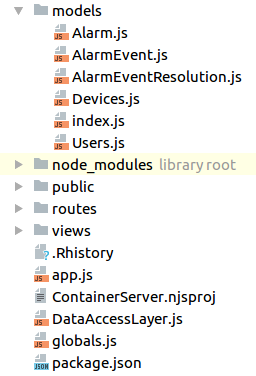
\includegraphics[scale=0.6]{gfx/structure}
\end{figure}
\smallskip

The overall structure can be seen on a following class diagram (please note that due to nature of node.js and reccommended practices for sequelize.js and express.js the OOP paradigm was not fully applied and hence the class diagram is bolted onto based on the file names and functions they define):
\bigskip
\begin{figure}[H]
\centering
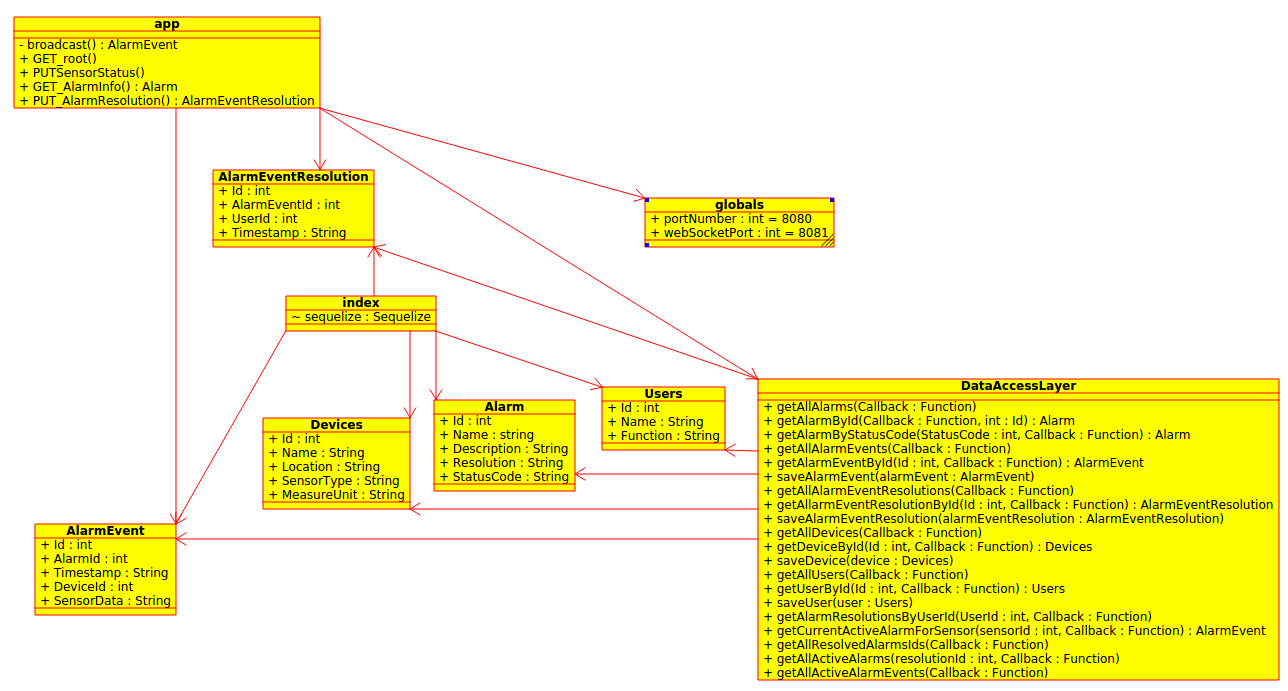
\includegraphics[scale=0.3]{gfx/class}
\end{figure}
\smallskip
As a short explanation to the class diagram above it is important to point out that the index.js file is picked up by sequelize at execution and hence it is not imported within any of the other files explicitely.

\smallskip

One final thing worth mentioning is presence of database deployment script that creates and initializes the database automatically. The script is an SQL Script with executor implemented as both bash and batch script hence it is possible to be executed on multiple environments. The script is present in the DBScripts folder in the root folder of the repository.
%%% Local Variables:
%%% mode: latex
%%% TeX-master: "../ClassicThesis"
%%% End:
